\section{Software Modularity}\label{sec:software-modularity}

Since software modularity is a key concept of our work, in this section we
spend a few pages reviewing important ideas related to it. First of all, it
is important to notice that the criteria used in this paper for
considering a modular design is based on the proposal of David Parnas~\cite{parnas-cacm-1972}.
Although proposed more than thirty years ago, these criteria are still used as
a guide for architects and has been applied in another areas. Based on
such criteria, modularity is closely related to design decisions that decompose
and organize the system into a set of modules.
Moreover, the following qualities attributes are expected in a modular design:

\begin{description}

\item[Comprehensibility] A modular design allows developers to
understand a module looking only at: (1) the implementation of the
module itself; and (2) the interfaces of the other modules
referenced by it.

%footnote{This comprehensibility degree is also
%known as \emph{modular reasoning}.}.

\item[Changeability] A modular design enables local
changes. If changes are necessary in the internal implementation of
a module \emph{A}, the other modules that depend exclusively on
\emph{A's interface} will not need to change, since there is no
modification in the module interface.

\item[Parallel development] After the specification of the module
interfaces, a modular design enables the parallel development of
modules. Different teams might only focus on their own modules
development, reducing the time-to-market and the need of
communication.

\end{description}

Parnas proposed the \emph{information hiding} principle as the
criteria to be used in decomposition of systems into modules.
According to Parnas, the parts of a system that are more likely to
changes must be hidden into modules with stable interfaces.

Recently, Baldwin and Clark~\cite{clark-design-rules-book} proposed a theory
which considers modularity as a key factor to innovation and market growth,
independent of the industry area. Their theory uses Design Structure Matrixes
(DSMs) to reason about dependencies among artifacts and argues that the task
structure of an organization is closely related to such dependencies. As a
consequence, if two modules are coupled, they can not be developed in
parallel, which actually requires either (a) more communication between
different teams; or (b) their implementation to be assigned to a single team.

In order to reason about modularity in this paper, we use Design Structure
Matrixes (DSMs) as a tool for visualizing dependencies among design parameters.
These parameters correspond to any decision that needs to be made along the
product design. Design parameters might have different abstraction levels. In
software industry, for example, some design decisions are related to process
development, language, code or architectural style, and so
forth~\cite{ribeiro-sbes-07}. Moreover, in this paper we also consider
implementation as a design activity. Therefore, software components like
classes, interfaces, packages, and aspects are also represented as design
parameters. We need to make several decisions about them.

Based on the DSM notation, a dependency arises whenever a design
decision depends on another. Such decisions, as explained earlier, are
represented as design parameters and disposed in both rows and columns of a
matrix. A dependency between two design decisions (or parameters) is represented
with a X in their corresponding lines and columns.

For example, suppose that the DSM depicted in Figure~\ref{dsm:example} represents
software components as parameters. The mark in row B, column A means that design
decisions regarded to component B depend on decisions concerned to the component
A. In a similar way, a X in row A, column B means that design decisions of
component A depend on decisions of component B. Whenever this mutual dependency
occurs, we have an occurrence of cyclical dependency, which in fact implies that
both components can not be independently addressed. As a consequence, their
parallel development is compromised.

\begin{figure}[h]
    \begin{center}
           \begin{scriptsize}
            \begin{tabular}{|l|l|l|l|} \hline
                       & A     & B     & C 	\\ \hline
                A      &       &  x    &   	\\ \hline
                B 	   &  x    &       &  x \\ \hline
                C	   &       &       &   	\\ \hline
            \end{tabular}
            \end{scriptsize}
            \label{dsm:example}
        \caption{Example of dependencies in a DSM.}
    \end{center}
\end{figure}

In the same DSM of Figure~\ref{dsm:example}, component B depends on C (expressed
by a X in row B, column C) but C does not depend on any other component (there is
no mark in row C). Therefore, C can be independently developed but B can not be
completely developed until design decisions of C have been concluded. In order to
improve modularity, i.e. removing some dependencies between design
decisions, several assumptions must be made before starting the design of a
parameter. Such assumptions, represented as a special kind of parameter,
were named by Baldwin and Clark~\cite{clark-design-rules-book} as Design Rules.

Therefore, Design Rules are parameters used as interfaces between modules that
are less likely to be changed~\cite{lopes-taosd-2006}. In this way, they can promote decoupling
of design parameters, like interfaces decrease the coupling between software
components. Such design rules establish strict partitions of knowledge and effort at the
outset of a design process. They are not just guidelines or recommendations: they must
be rigorously obeyed in all phases of design and production~\cite{clark-design-rules-book}.
Figure~\ref{dsm:example-drs} illustrates components A and B being decoupled
by using design rules. Since A and B do not depend each other anymore, it is possible
for example to change A for A' as long as A' respects the design rule. In addition,
when both respect the design rules, the parallel development becomes possible. However, notice
that the coupling does not disappear. Its place has been changed instead: A is coupled
to the design rule. The same happens to B.

\begin{figure}[h]
    \begin{center}
           \begin{scriptsize}
            \begin{tabular}{|l|l|l|l|l|} \hline
                        & DRs    & A     & B    & C  \\ \hline
                DRs     &        &       &   	&    \\ \hline
                A       &  x     &       &   	&    \\ \hline
                B 	    &  x     &       &   	& x  \\ \hline
                C	    &        &       &   	&    \\ \hline
            \end{tabular}
            \end{scriptsize}
            \label{dsm:example-drs}
        \caption{Design Rules decoupling components A and B.}
    \end{center}
\end{figure}

\section{Modularity Issues in Aspect-Oriented Programming}\label{sec:aop-issues}

Aspect-Oriented Programming was proposed to modularize crosscutting
concerns~\cite{kiczales-ecoop-1997}. However, constructions supported by
AspectJ~\cite{kiczales-cacm-2001} like languages can produce high
coupling between the base code and the aspects, which may compromise
the aforementioned modular criteria. In this section, we illustrate
this problem through some examples, which were primarily extracted from
the Health Watcher system~\cite{soares-oopsla-02}.

Health Watcher (HW) is a real web-based information system
originally implemented in Java and restructured to use AspectJ
\cite{kiczales-cacm-2001}. The system was developed to improve the quality
of the services provided by health care institutions, allowing citizens
to register complaints regarding health issues, and heath care
institutions to investigate and take the required actions.

We have selected the HW system because its design has a significant number of
non-crosscutting and crosscutting concerns. Furthermore, it requires a number of
common day-to-day design decisions related to GUI, persistence, and concurrency.
Finally, the HW system has been used as a case study in several
\emph{aspect-oriented} works~\cite{greenwood-ecoop-2007, greenwood-ea-2007,
soares-oopsla-02}.

\begin{figure}[t]
\centering
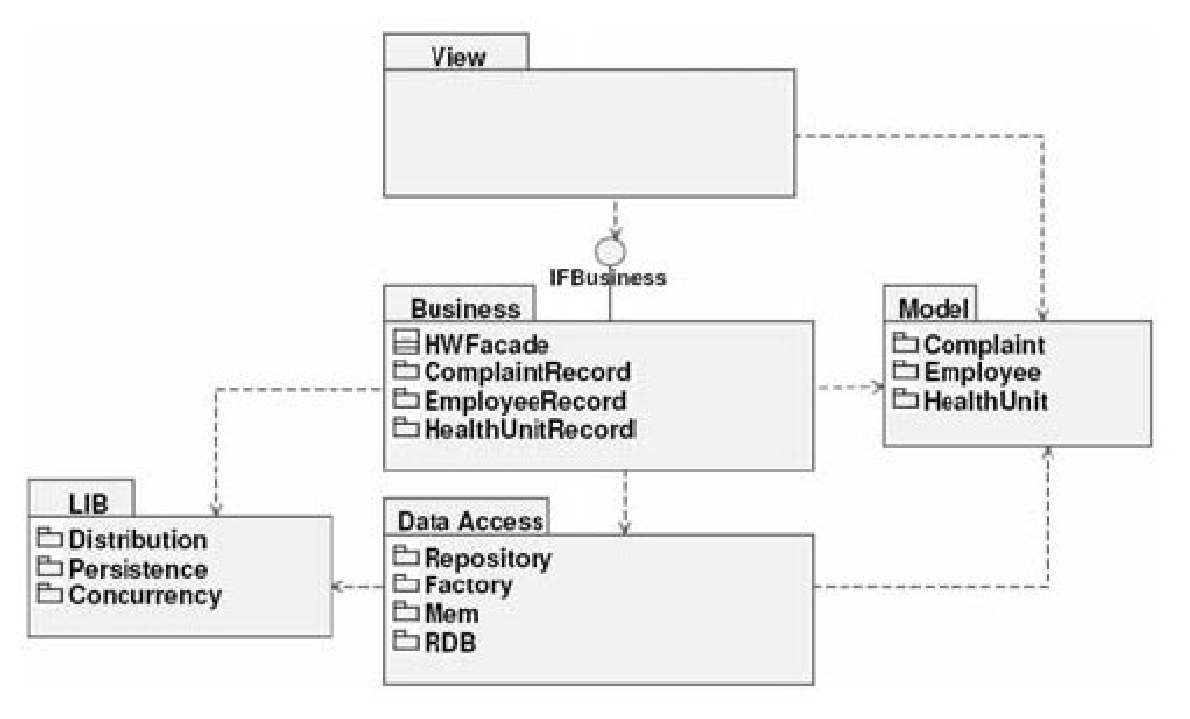
\includegraphics[scale=0.5]{images/hw.eps}
\caption{Overview of the Health Watcher architecture.}
\label{fig:hw-architecture}
\end{figure}

Figure~\ref{fig:hw-architecture} shows the base architecture of the
HW system. This architecture aims at modularizing user interface,
distribution, business rules, and data management concerns. Below
we describe the major architectural components of the HW system:

\begin{description}
\item [View Layer:] related to the HW web interface. The
implementation of this layer is based on Front
Controller~\cite{alur-book-2003} and
Command~\cite{gamma-dpbook-1995} patterns, using \emph{servlets}
and \emph{plain Java objects}. The communication with the business layer
is implemented with calls to the \emph{IFBusiness}, which may be
distributed or not.

\item [Business Layer:] responsible for business
logic and transactional concern implementation. The
\emph{HWFacade}, which implements \emph{IFBusiness}, is the unique
point of interaction with this layer. This class uses
\emph{record} components to interact with the Data Access Layer.

\item [Data Access Layer:] responsible for abstracting the persistence
mechanism following the Data Access Object
pattern~\cite{alur-book-2003}. Some interfaces to
manage data persistence are defined in this layer. Two
implementations are available: the first one uses volatile memory
whereas the second one is based on relational databases.

\item [Model:] responsible for implementing the \emph{domain objects}.
These objects represent the core concepts of the application;
transit between all architectural layers; and have a few
implementation logic. \emph{Complaint}, \emph{employee}, and \emph{health unit}
are examples of core concepts in the HW system.

\item [Lib Components:] represent reusable components that are useful
to the implementation of concerns like persistence, distribution,
and concurrency.
\end{description}

In what follows, we present several issues related to \emph{aspect-oriented}
modularity. First, we discuss the problem of unanticipated changes
in base code --- problem named as fragile pointcut in the \emph{aspect-oriented} community. After that,
we argue that clear interfaces, for decoupling crosscutting code from base
code, are necessary for developing different concerns in parallel.

\subsection{Unanticipated Changes in Base Code}

%%%%%%%%%%%%%%%%%%%%%%%%%%%%%%%%%%%%%%%%%%%%%%%%%%%%%%%%%%%%%%%%%%%%%%%%%%%%%%
% Realmente, estas duas se��es podem n�o ter uma separa��o...

% Aqui, fala-se de fragile. No segundo exemplo tamb�m. Aqui, a gente
% sup�e um desenvolvedor da classe  "not aware" sobre os aspectos, mas que
% n�o deixa de ser um problema de paralelismo. O desenvolvimento em
% paralelo � discutido no segundo exemplo... n�o sei n�o, mas talvez seja
% melhor n�o fazer essas separa��es... (pelo menos foi essa a impress�o que
% eu tive hoje). Talvez seja bom atacarmos algo mais geral: "problemas de modularidade..."
%%%%%%%%%%%%%%%%%%%%%%%%%%%%%%%%%%%%%%%%%%%%%%%%%%%%%%%%%%%%%%%%%%%%%%%%%%%%%%

In this section, we present an example of unanticipated changes in the base code.
We aim at showing that, when unanticipated changes happens, the aspects might not
work as presumed.

Consider the transaction management concern, which requires that certain methods
of the HW buisiness layer must deal with transactional behavior. The
implementation of such a concern consists of encompassing these methods with
transactional blocks. Listing~\ref{lst:ao-transaction} illustrates the source 
code related to this concern in AspectJ.

\scriptsize
\begin{lstlisting}[frame=single, caption={Aspect responsible for implementing the transactional concern.},label=lst:ao-transaction, language=Java]
public aspect TransactionAspect {

    public pointcut transactionalMethods() : /* ... */
 
	before() : transactionalMethods() {
		persitentMechanism.beginTransaction();	    
	}

	after() : transactionalMethods() {
		persistentMechanism.commitTransaction();
	}

	after() throwing : transactionalMethods() {
		persistentMechanism.rollBack();
	}

}
\end{lstlisting}

\normalsize

% Now, suppose a new feature intended to count the number of employees
% registered in a given profile. Such a feature might be implemented as
% a new method in the \emph{EmployeeRepository} class
% (Listing~\ref{lst:new-method}).
% 
% \scriptsize
% \begin{lstlisting}[frame=single, caption={A new method for counting the number of Employees.},label=lst:new-method, language=Java]
% public class EmployeeRepository {
% 
%     public void insertEmployee(Employee employee) { ... }
% 
%     public void removeEmployee(Employee employee) { ... }
% 
%     public int getNumberOfEmployees(Profile profile) {
%         // Business logic to count the number of Employees
%     }
% 
% }
% \end{lstlisting}
% \normalsize

If a class developer {\bf is} oblivious about the
\emph{TransactionAspect} aspect decides to implement a 
new transactional method (\emph{newMethod()}), at least two 
problems might occur:

\begin{enumerate}

    \item if the method created by the class does not implement the
    transactional block and does not expose the join point matched by the 
    \emph{transactionalMethod()} pointcut, the method will not work 
    as being a transactional behavior;

    \item if the class developer, oblivious about the aspect,
    implements the transactional management concern in the
    new method, and this method is matched by the \emph{transactionalMethod()}
    pointcut, an expected behavior might occur, since two consecutive 
    calls to \emph{beginTransaction()} are made. 
\end{enumerate}


The situation above exposes that problems of modularity have
occurred: (1) the comprehensibility is compromised, since two
modules should be studied in order to understand the concern; and
(2) the parallel development is problematic, because one developer
can implement unintended behavior into a module which, although it
is not under his responsibility, might break the system.

Therefore, we conclude that any unanticipated change in the class
may cause problems and the application might not behave as presumed.
Notice that we have a cyclical dependency situation: the aspect
depends on the class syntactically; and to change the class, the
developer must be aware about the aspect.
Figure~\ref{dsm:concurrency} illustrates such a cyclical
dependency through a DSM (presented in Section~\ref{sec:software-modularity}), whereas
Figure~\ref{dsm:concurrency-drs} shows design rules coming into
play to remove the dependency between the aspect and class.

\begin{figure}[h]
    \begin{center}
        \subfigure[Cyclical Dependency between an aspect and a class.] {
            \begin{scriptsize}
            \begin{tabular}{|l|l|l|l|} \hline
                  &                             & 1     & 2     \\ \hline
                1 & TransactionAspect.aj    & \paintcell     & x     \\ \hline
                2 & Business java classes     & x     & \paintcell      \\
                \hline
            \end{tabular}
            \end{scriptsize}
            \label{dsm:concurrency}
        }
        \subfigure[Design Rules removing Cyclical Dependency.] {
            \begin{scriptsize}
            \begin{tabular}{|l|l|l|l|l|} \hline
                  &                             & 1     & 2    & 3 \\ \hline
                1 & Design Rules                &       &      &   \\ \hline
                2 & TransactionAspect.aj    & x     &      &   \\ \hline
                3 & Business java classes     & x     &      &   \\ \hline
            \end{tabular}
            \end{scriptsize}
            \label{dsm:concurrency-drs}
        }
        \caption{Transaction concern with/without Design Rules.}
    \end{center}
\end{figure}

In summary, this problem reveals to us that we need interfaces (or design
rules) that forbid calls to certain methods within the business class (eg.
\emph{beginTransaction()}, \emph{commitTransaction()}, and \emph{rollBack()})
and expose which are the expected signature of methods to be matched by 
the \emph{transactionalMethods} pointcut.

\subsection{Unsupported Parallel Development}

Another example of modularity issue might arise when a team is
assigned to develop a crosscutting concern and another team is
assigned to develop the base concerns of a system. In order to
reduce the time-to-market, it may be desirable to develop both
concerns in parallel. However, without the use of a clear interface
between those concerns, a lot of communication might be required,
which, in fact, compromises the parallel development.

When reasoning about modularity in software engineering,
the benefit of parallel development is frequently not considered, even after
Parnas claimed that modularity is more than program structure. Actually,
his view regarding modularity is related to the assignment of development
activities, which, of course, may be reflected in the program
structure~\cite{parnas-icse-03}. A similar view of modularity was presented by Baldwin and
Clark~\cite{clark-design-rules-book},  since they
reported that a modular design reduces the communication paths among
design decisions, in such a way that unities of work can be developed
in parallel.

% \begin{quote}\emph{
% My early work clearly treated modularization as a design
% issue, not a language issue. A module was a work assignment,
% not a subroutine or other language element. Although
% some tools could make the job easier, no special tools were
% needed to use the principal, just discipline and skill.}
% (D. Parnas)
% \end{quote}


% include the parnas review of modularity
% read a bit more about the steimann discussion on AOP modularity
% we need a clear interface for both aspect and base code....



For instance, suppose that a team is responsible for developing
the use cases related to the \emph{complaint management} concern (a core concern
of Health Watcher system); and another team is responsible
for an auditing concern that must be triggered whenever a change in a
complaint occurs. Without a clear interface stating which are the relevant
complaint changes (the set of join-points) and how these join-points should be
written by the complaint management team, any increment in the core concern
must be communicated to the auditing team. Consequently, it is difficult to
implement the auditing concern at the same time that the complaint management
concern is being developed. Although these concerns can be encapsulated in
single unities, there is no modular design in this case.

In what follows, consider the DSM depicted in Figure~\ref{dsm:hw01}, which represent
some design parameters and respective dependencies of the Health Watcher
system. Based on this DSM, we can realize that decisions regarded to the
complaint implementation (row 5) depend on decisions about complaint
requirements (dependency row 5, column 2), about architectural
decisions\footnote{Examples of architectural decisions for the Health Watcher
system are the selected style (layers), patterns, and technologies for each
layer or concern (presentation, distribution, persistence, and so on.)}
(dependency row 5, column 4), and about the auditing concern (dependency row 5,
column 6). This last dependency occurs because the team responsible for developing
the \emph{complaint concern} have to know how to develop the extension points for
the \emph{auditing concern}. Moreover, as we can observe in
Figure~\ref{dsm:hw01}, the auditing implementation also depends on the
complaint implementation decisions, since changes in its implementation should
be notified to the auditing implementation team. In this way, there is a
cyclical dependency between complaint implementation and auditing
implementation -- a clear example of non modular design.

\begin{figure}[htb]
\centering
\begin{scriptsize}
\begin{tabular}{|l|l|l|l|l|l|l|l|} \hline
  &                             & 1     & 2     & 3     & 4     & 5     & 6 \\ \hline
1 & Goals and constraints       &       &       &       &       &       &   \\ \hline
2 & Complaint requirements      & x     &       &       &       &       &   \\ \hline
3 & Auditing requirements       & x     &       &       &       &       &   \\ \hline
4 & Architectural decisions     & x     & x     &       &       &       &   \\ \hline
5 & Complaint implementation    &       & x     &       & x     &       & x \\ \hline
6 & Auditing AO implementation  &       &       & x     &       & x     &   \\  \hline
\end{tabular}
\end{scriptsize}
\caption{DSM Analysis Health Watcher}
\label{dsm:hw01}
\end{figure}

% Now, let's look at the source code of this example. Listing~\ref{lst:complaint-repository}
% illustrates the ComplaintRepository class. Suppose that the auditing concern must be
% triggered when inserting, removing, updating, or searching for a complaint.
% 
% \scriptsize
% \begin{lstlisting}[frame=single, caption={Complaint Repository implementation.},label=lst:complaint-repository, language=Java]
% public class ComplaintRepository implements IComplaintRepository {
% 
%     public int insert(Complaint c) throws RepositoryException,
%             ObjectAlreadyInsertedException {
% 
%     }
% 
%     public void update(Complaint c) throws RepositoryException,
%             ObjectNotFoundException {
% 
%     }
% 
%     public void remove(int id) throws RepositoryException,
%             ObjectNotFoundException {
% 
%     }
% 
%     public Complaint search(int id) throws RepositoryException,
%             ObjectNotFoundException {
% 
%     }
% 
% }
% \end{lstlisting}
% \normalsize
% 
% Remember that two teams are working in parallel without design rules: the first one
% works on the base code (ComplaintRepository) and the second one
% works on the auditing concern. Such a concern is implemented as an
% aspect (Listing~\ref{lst:auditing-aspect}).
% 
% \scriptsize
% \begin{lstlisting}[frame=single, caption={Auditing Aspect.},label=lst:auditing-aspect, language=Java]
% public aspect AuditingAspect {
% 
%     pointcut auditWhen():
%            execution(int ComplaintRepository.insert(Complaint)
%         || execution(void ComplaintRepository.update(Complaint)
%         || execution(void ComplaintRepository.remove(int)
%         || execution(Complaint ComplaintRepository.search(int)
% 
%     after() returning(): auditWhen() {
%         // audit code.
%     }
% 
% }
% \end{lstlisting}
% \normalsize
% 
% In the meanwhile, when the teams are working on their
% respective concerns, for some reason the team of the repository changed the following:
% (i) the insert method now returns void instead of int; and (ii) the remove method
% take as parameter a Complaint object instead of an id. Obviously, such changes might
% break the aspects and the auditing concern will not work correctly.

Based on the information hiding principle, we should encapsulate the
dependencies between complaint and auditing concerns in a special kind
of interface (a design rule).
Applying design rules to this example, we improve the design structure
by removing the cyclical dependencies between complaint and auditing concerns.
The reviewed DSM is presented in Figure~\ref{dsm:hw02}. Notice that a new parameter
(actually a design rule) was introduced (row 5) and all dependencies are bellow
the main diagonal (there is no more cyclical dependencies). This design rule
was proposed in order to improve the parallel development between class
developers and aspect developers. Actually, it is responsible to
establish contracts that define what is expected from both teams.

\begin{figure}[htb]
\centering
\begin{scriptsize}
\begin{tabular}{|l|l|l|l|l|l|l|l|l|} \hline
  &                                 & 1     & 2     & 3     & 4     & 5     & 6 & 7 \\ \hline
1 & Goals and constraints           &       &       &       &       &       &   &   \\ \hline
2 & Complaint requirements          & x     &       &       &       &       &   &   \\ \hline
3 & Auditing requirements           & x     &       &       &       &       &   &   \\ \hline
4 & Architectural decisions         & x     & x     &       &       &       &   &   \\ \hline
5 & Auditing design rule            &       & x     &   x   &       &       &   &   \\ \hline
6 & Complaint implementation        &       & x     &       &   x   & x     &   &   \\ \hline
7 & Auditing AO implementation      &       &       &   x   &       & x     &   &   \\ \hline
\end{tabular}
\end{scriptsize}
\caption{DSM Analysis Health Watcher}
\label{dsm:hw02}
\end{figure}

Existing works, such as \emph{Open Modules}~\cite{aldrich-ecoop-05},
propose the use of interfaces for exposing \emph{joinpoints} in the base code, which, in fact,
defines the responsibilities just for class developers, besides limiting the scope of advised code.
Therefore, existing approaches do not offer mechanisms for describing the responsibilities of aspect developers.
As a consequence, class developers are still able to implement part of a concern
assigned for a different team and they can not assume the existence
of any behavior expected to be modularized as an aspect.

% Acho que podemos tirar esse exemplo de jogos e colocar o c�digo de auditing no exemplo acima
% (ou seja, pegar o c�digo da se��o 5 e colocar aqui...)

% For instance, consider the implementation of a mobile
% game product line. Listing~\ref{lst:paint-method} presents part of
% a non-variant code responsible for painting graphical elements
% on the screen. Methods \emph{paintBeforeScrolling} and
% \emph{paintScolling} are introduced (by means of intertype declararions),
% and represent variation points that should be implemented as aspects for each
% target device. To our knowledge, there is no approach for specifying that such methods must be called
% within the \emph{paint} method and that they must be introduced by aspects.
% 
% \scriptsize
% \begin{lstlisting}[frame=single, caption={Dependency of a base code to an aspect code.},label=lst:paint-method, numbers=left, language=Java]
%  public void paint(Graphics g) {
% 	Enemy myEnemy = null;
% 	int i = 0;
% 	int j = 0;
% 	g.setClip(0, 0, Resources.CANVAS_WIDTH, Resources.CANVAS_HEIGHT);
% 	paintBeforeScrolling(g);
% 	if (this.scroll.isScrolling) {
% 	 	paintScrolling(g);
% 	} else if (!isGameOver){
% 	 ...
% \end{lstlisting}
% 
% \normalsize

